\subsection{Transience of the second order remainder structure}
\label{sec:trans-second-order}

In this section we demonstrate a theoretical property of the state
learner which is useful for targeted learning (c.f., Section
\ref{sec:targeted-learning}). Specifically we consider an estimator of
a target parameter which is obtained by substituting the state learner
estimates of the nuisance parameters $\Lambda_1$, $\Lambda_2$, and
$\Gamma$. An example is an estimator of the cumulative incidence
curve, which can be obtained from estimators of $\Lambda_1$ and
$\Lambda_2$. Another example is provided in Section \ref{sec:targeted-learning}.
By equations~(\ref{eq:lambdaj}) and~(\ref{eq:gamma}) and the definition of
\( F \), we have
\begin{equation}
  \label{eq:7}
  \Gamma(t , x) 
  = \int_0^t  \frac{F(\diff s, -1, x )}{F(s-, 0, x )},
  \quad \text{and} \quad
  \Lambda_j(t , x) 
  = \int_0^t  \frac{F(\diff s, j, x )}{F(s-, 0, x )},
  \quad j \in \{1,2\},
\end{equation}
and thus an estimator based on \( \hat{\Lambda}_{1,n} \),
\( \hat{\Lambda}_{2,n} \), and \( \hat{\Gamma}_{n} \) can also be obtained from
an estimator of $F$ using equation~(\ref{eq:7}). A so-called targeted estimator
has the key feature that it is asymptotically equivalent to a sum of i.i.d.\
random variables plus a second order remainder term
\citep{van2011targeted,hines2022demystifying}. For the setting with competing
risks, the remainder term is dominated by terms of the form
\begin{equation}
  \label{eq:dr-term}
  P{\left[
      \int_0^{\tau} w_n(s, \blank)
      \hat{M}_{1,n}(s \mid  \blank)
      \hat{M}_{2,n}(\diff s \mid  \blank)
    \right]},
\end{equation}
where \( (\hat{M}_{1,n}, \hat{M}_{2,n}) \) is any of the nine combinations of
\( \hat{M}_{1,n} \in \{[\Gamma -\hat{\Gamma}_n], [\Lambda_1
-\hat{\Lambda}_{1,n}], [\Lambda_2 -\hat{\Lambda}_{2,n}]\} \) and
\( \hat{M}_{2,n} \in \{[\Gamma -\hat{\Gamma}_n], [\Lambda_1
-\hat{\Lambda}_{1,n}], [\Lambda_2 -\hat{\Lambda}_{2,n}]\} \), and \( w_n \) is
some data-dependent function with domain \([0,\tau]\times\mathcal X \)
\citep{van2003unified}. In particular, a targeted estimator will be
asymptotically linear if the `products' of the estimation errors
\( \hat{M}_{1,n} \) and \( \hat{M}_{2,n} \) in equation~(\ref{eq:dr-term}) are
\( \smallO_P{(n^{-1/2})}\). Proposition~\ref{prop:dr-structure} states that if
equation~(\ref{eq:dr-term}) holds for a targeted estimator based on estimators
$\hat{\Lambda}_{1,n}$, $\hat{\Lambda}_{2,n}$, and $\hat{\Gamma}_{n}$, then a
similar product structure holds for a targeted estimator based on
\( \hat{F}_n \). We state the result for the special case that
\(\hat{M}_{1,n}= \Gamma-\hat{\Gamma}_n \) and
\(\hat{M}_{2,n} =\Lambda_1-\hat{\Lambda}_{1,n} \), but similar results hold for
any combinations of \( \Gamma-\hat{\Gamma}_n\),
\( \Lambda_1-\hat{\Lambda}_{1,n} \), and \( \Lambda_2-\hat{\Lambda}_{2,n} \).
\begin{proposition}
  \label{prop:dr-structure}
  Assume that \( w(s,x)\leq c \), \( F(s, 0, x) \geq 1/c \) and
  \( \hat{F}_n(s, 0, x) \geq 1/c \) for some \( c>0 \) for all
  \( s \in [0, \tau] \) and \( x \in \mathcal{X} \). Then there are real-valued
  uniformly bounded functions \( w^a_n \), \( w^b_n \), \( w^c_n \), and
  \( w^d_n \) with domain \( [0,\tau]^2 \times \mathcal{X} \) such that
  \begin{align*}
    & P{\left[
      \int_0^{\tau} w(s, \blank)
      \left\{
      \Gamma(s,\blank) -\hat{\Gamma}_n(s,\blank)
      \right\}
      [\Lambda_1-\hat{\Lambda}_{1,n}]
      (\diff s, \blank)
      \right]}
    \\
     & =
      P{\big[
      \int_0^{\tau} \int_0^{s} w^a_n(s,u,\blank) [F - \hat{F}_n](u-, 0,
       \blank)[F - \hat{F}_n](s-, 0, \blank)}
    \\
    & \qquad \quad \times F(\diff u, -1, \blank ) F ( \diff s, 1, \blank)
      \big]
    \\
    & \quad +
      P{\left[
      \int_0^{\tau} \int_0^{s} w^b_n(s,u,\blank) [F - \hat{F}_n](u-, 0, \blank)
      F(\diff u, -1, \blank ) [F - \hat{F}_n](\diff s, 1, \blank)
      \right]}
    \\
    & \quad +
      P{\left[
      \int_0^{\tau} \int_0^{s} w^c_n(s,u,\blank) [F - \hat{F}_n](\diff u, -1, \blank)
      [F - \hat{F}_n](s-, 0, \blank)
      F(\diff s, 1, \blank ) 
      \right]}
    \\
    & \quad +
      P{\left[
      \int_0^{\tau} \int_0^{s} w^d_n(s,u,\blank) [F - \hat{F}_n](\diff u, -1, \blank)
      [F - \hat{F}_n](\diff s, 1, \blank)
      \right]}.
  \end{align*}
\end{proposition}
\begin{proof}
  See Appendix~\ref{sec:state-learner-with}.
\end{proof}


\section{Targeted learning}
\label{sec:targeted-learning}

In this section, we consider a suitably smooth operator
\( \theta \colon \mathcal{Q} \rightarrow \Theta \) which represents a
target parameter of interest. The parameter space $\Theta$ can be a
subset of \(\R^d\) or a subset of a function space, for example a
subset of \(\mathcal{M}_{\tau}\) as in Section
\ref{sec:super-learning}. In subsection~\ref{sec:cause-spec-aver} we
discuss an example from causal inference where $\theta$ is the average
treatment effect and \( \Theta = [-1,1] \).  To discuss the role of
the state learner for targeted learning we briefly review some results
from semiparametric efficiency theory. Extensive reviews and
introductions are available elsewhere
\cite[e.g.,][]{pfanzagl1985contributions,bickel1993efficient,van2003unified,tsiatis2007semiparametric,kennedy2016semiparametric}.
Under the assumption of conditional independent censoring and
positivity, $\theta$ is identifiable from \( \mathcal{P} \) which
means that there exists an operator
\( \Psi \colon \mathcal{P} \rightarrow \Theta \) such that
\( \theta(Q) = \Psi(P_{Q, \Gamma}) \) for all
$\Gamma \in \mathcal{M}_{\tau}$.  By equation~(\ref{eq:parametrizeP})
this implies that we may write
\begin{equation*}
  \theta(Q) = \Psi(P) = \tilde{\Psi}^0(\Lambda_1, \Lambda_2, H),
\end{equation*}
for some operator \( \tilde{\Psi}^0 \). The state learner provides a ranking of
all tuples
\( (a_1, a_2, b) \in \mathcal{A}_1 \times \mathcal{A}_2 \times \mathcal{B} \).
We use \( \hat{a}_{1,n} \), \( \hat{a}_{2,n} \), and \( \hat{b}_n \) to denote
the learners corresponding to the discrete state learner \( \hat{\phi}_n \),
i.e., the tuple with the highest rank. Letting \( H_n(\data_n) \) denote the
empirical measure of \( \{X_1, \dots, X_n\} \), we obtain a plug-in estimator of
$\theta$:
\begin{equation}
  \label{eq:2}
  \hat{\Psi}^0(\data_n) =
  \tilde{\Psi}^0(\hat{a}_{1,n}(\data_n), \hat{a}_{2,n}(\data_n), H_n(\data_n)). 
\end{equation}

The asymptotic distribution of \( \hat{\Psi}^0 \) is
difficult to analyse due to the cross-validated model selection step
involved in the estimation of the nuisance parameters $\Lambda_1$ and
$\Lambda_2$.
% In addition, the estimator will typically have an
% asymptotic bias that vanishes at a too slow 
% rate.
Using tools from semi-parametric efficiency theory, it is possible to
construct a so-called targeted or debiased estimator with an
asymptotic distribution which we know how to estimate
\citep{bickel1993efficient,van2011targeted,chernozhukov2018double}. A
targeted estimator is based on the efficient influence function for
the parameter $\tilde{\Psi}^0$ and relies on estimators of the
nuisance parameters $\Gamma$, \( \Lambda_1 \) and $\Lambda_2$. The
efficient influence function is a \( P \)-zero mean and square
integrable function which we denote by
\( \psi(\blank ; \Lambda_1, \Lambda_2, \Gamma) \). The name is
justified because any regular asymptotically linear estimator that has
\( \psi \) as its influence function is asymptotically efficient,
meaning that it has smallest asymptotic variance among all regular
asymptotically linear estimators \citep{bickel1993efficient}.

An example of a targeted estimator is the one-step estimator, defined as
\begin{equation}
    \label{eq:one-step-def}
    \begin{split}
      \hat{\Psi}_{\text{OS}}(\data_n)
      = &
          \tilde{\Psi}^0(\hat{a}_{1,n}(\data_n), \hat{a}_{2,n}(\data_n),
          H_n(\data_n))
      \\
        & + \empmeas{[\psi(\blank; \hat{a}_{1,n}(\data_n), \hat{a}_{2,n}(\data_n),
          \hat{b}_n(\data_n) )]},
    \end{split}
\end{equation}
where \( \empmeas \) is the empirical measure of a data set
\(\{O_i\}_{i=1}^n\).
Under suitable regularity conditions
we have the
following asymptotic expansion of the one-step estimator
\citep{pfanzagl1985contributions,van2003unified,fisher2021visually,kennedy2022semiparametric},
\begin{equation*}
  \hat{\Psi}_{\text{OS}}(\data_n)- \Psi(P)
  =  \empmeas{[\psi(\blank ; \Lambda_1, \Lambda_2, \Gamma)]}
  +\mathrm{Rem}{(\hat{\Lambda}_{1,n},\hat{\Lambda}_{2,n},  \hat{\Gamma}_n, P)} + \smallO_{P}(n^{-1/2}),
\end{equation*}
where the remainder term has the form
\begin{equation}
  \label{eq:4}
  \mathrm{Rem}{(\hat{\Lambda}_{1,n},\hat{\Lambda}_{2,n},  \hat{\Gamma}_n, P)}
  = \bigO_P{
    \left\{
      \|\Lambda_1-\hat{\Lambda}_{1,n}\|^2
      +
      \|\Lambda_2-\hat{\Lambda}_{2,n}\|^2
      +
      \|\Gamma-\hat{\Gamma}_{n}\|^2
    \right\}
  },
\end{equation}
for some suitable norm \( \|\blank \| \), for instance the
\( \mathcal{L}_{P}^2 \)-norm. When equation~(\ref{eq:4}) holds and the
nuisance parameters $\Lambda_1$, $\Lambda_2$, and $\Gamma$ are
consistently estimated at rate \( \smallO_P{(n^{-1/4})} \), then
\begin{equation}
  \label{eq:3}
  \sqrt{n}(\hat{\Psi}_{\text{OS}}(\data_n)- \Psi(P)) \weakly \mathcal{N}(0,
  P{[\psi(\blank; \Lambda_1, \Lambda_2, \Gamma)^2]}),
\end{equation}
where we use \( \weakly \) to denote weak convergence \citep{van2000asymptotic}.
In particular, equation~(\ref{eq:3}) and Slutsky's lemma imply that we can
obtain asymptotically valid \((1-\alpha)\cdot100\%\) confidence intervals by
calculating
\begin{equation*}
  \left[
    \hat{\Psi}_{\text{OS}}(\data_n) - q_{\alpha/2} \hat{\sigma}(\data_n) ,
    \;
    \hat{\Psi}_{\text{OS}}(\data_n) + q_{\alpha/2} \hat{\sigma}(\data_n)
  \right],
\end{equation*}
where \( q_{\alpha} \) is the \( (1-\alpha) \)-quantile of the standard normal
distribution and
\begin{equation*}
  \hat{\sigma}(\data_n)^2 = \empmeas{ \left[ \psi(\blank;
      \hat{a}_{1,n}(\data_n), \hat{a}_{2,n}(\data_n), \hat{b}_n(\data_n))^2
    \right]}.
\end{equation*}



\subsection{Average treatment effect on the absolute risk of an event}
\label{sec:cause-spec-aver}

In the following we detail how the state learner can be used to
construct a targeted estimator of the cause-specific average treatment
effect \citep{rytgaard2022targeted}. We assume that the covariate
vector \( X \in \R^p \) contains a binary treatment indicator \( A \)
and a vector of potential confounders,
\( W \in \mathcal{W}\subset \R^{p-1} \).  We use $\mu$ to denote the
marginal distribution of \( W \) and $\pi$ to denote the conditional
probability of treatment,
\begin{equation*}
  \pi(w) = P(A=1 \mid W=w).
\end{equation*}
We assume throughout that $\pi$ is uniformly bounded away from \( 0 \)
and \( 1 \) on \( \mathcal{W} \) and that both \( A \) and \( W \) are
fully observed for all individuals. We use a super learner to
estimate $\pi$ \citep{Polley_Ledell_Kennedy_Laan_2023_Superlearn}, and
we denote this estimator by $\hat{\pi}_n$. We use the empirical
measure of \( \{W_1, \dots, W_n\} \) to estimate $\mu$, and denote
this estimator by $\hat{\mu}_n$. As parameter of interest we consider
the standardised difference in the absolute risk of an event with
cause 1 at time $\tau$:
\begin{align*}
  & \theta_{{\tau}}(Q)
  \\
  & = \int_{\mathcal{W}} 
    \left\{
    \int_0^{\tau}
    S(s- \mid w, 1)  \Lambda_1(\diff s \mid w, 1)
    -
    \int_0^{\tau}
    S(s- \mid w, 0)  \Lambda_1(\diff s \mid w, 0)
    \right\}
    \mu(\diff w).
\end{align*}
Under the usual assumptions for causal inference (consistency,
positivity, no unmeasured confounding) \( \theta_{{\tau}} \) can be
given the causal interpretation
\begin{equation*}
  \theta_{{\tau}}(Q) =
  P{(T^{1} \leq \tau, D^{1}=1)}-
  P{(T^{0} \leq \tau, D^{0}=1)},
\end{equation*}
where \( (T^a, D^a) \), \( a \in \{0,1\} \), denote potential outcomes
\citep{hernanRobinsWhatIf}. In this case, the interpretation of $\theta_{\tau}$
is the difference in the average risk of cause \( 1 \) occurring before time
\( \tau \) in the population if everyone had been given treatment (\( A=1 \))
compared to if no one had been given treatment \( (A=0) \).

Using equation~(\ref{eq:surv-def}) we may write
\( \theta_{{\tau}}(Q) = \tilde{\Psi}_{\tau}^0(\Lambda_1, \Lambda_2, \mu) \), where
\begin{equation}
  \label{eq:1}    
  \begin{split}
    & \tilde{\Psi}_{\tau}^0(\Lambda_1, \Lambda_2, \mu)
    \\
    & =
      \int_{\mathcal{W}} 
      \int_0^{\tau}
      \exp{\{{-\Lambda_1(s- \mid w, 1)-\Lambda_2(s- \mid w, 1)}\}}  \Lambda_1(\diff s \mid
      w, 1)
      \mu(\diff w)
    \\
    &  \quad
      -\int_{\mathcal{W}} 
      \int_0^{\tau}
      \exp{\{{-\Lambda_1(s- \mid w, 0)-\Lambda_2(s- \mid w, 0)}\}}  \Lambda_1(\diff s \mid w, 0)
      \mu(\diff w).
  \end{split}
\end{equation}
The efficient influence function for the parameter $\tilde{\Psi}_{\tau}$ depends
on the set \( (\Lambda_1, \Lambda_2, \Gamma, \pi) \) of nuisance parameters.
We define
\begin{align*}
  \omega_a(A,W; \pi)
  &=  \frac{% (-1)^{a+1}
    \1{\{A=a\}}}{\pi(W)^{a}(1-\pi(W))^{1-a}},
  \\
  g(t, A, W; \Lambda_1, \Lambda_2)
  & = \int_0^{t}
    \exp{\{ {-\Lambda_1(s- \mid W, A)-\Lambda_2(s- \mid W, A)} \}}  \Lambda_1(\diff s \mid
    W, A),
  \\  
  M_j(\diff t \mid A, W;  \Lambda_j  )
  & = N_j(\diff t) -
    \1{\{\tilde{T} \geq t\}} \Lambda_j(\diff t \mid W, A),
    \quad j \in \{1,2\},
    \intertext{and}
    M(\diff t \mid A, W;  \Lambda_1, \Lambda_2  )
  & = M_1(\diff t \mid A, W;  \Lambda_1  ) +
    M_2(\diff t \mid A, W;  \Lambda_2  ).
\end{align*}
The efficient influence function can now be written as
\citep{van2003unified,jewell2007non,rytgaard2022targeted},
\begin{equation*}
  \psi_{\tau}(O; \Lambda_1, \Lambda_2, \Gamma, \pi)
  = \psi_{\tau}^1(O; \Lambda_1, \Lambda_2, \Gamma, \pi)
  - \psi_{\tau}^0(O; \Lambda_1, \Lambda_2, \Gamma, \pi)
  -\tilde{\Psi}_{\tau}^0(\Lambda_1, \Lambda_2, \mu),
\end{equation*}
where
\begin{equation}
  \label{eq:5}
  \begin{split}
    & \psi_{\tau}^a(O; \Lambda_1, \Lambda_2, \Gamma, \pi)
    \\
    & =
      \omega_a(A,W; \pi)
      \int_0^{\tau} \exp{\{{\Gamma(t- \mid A, W)}\}}   
      M_1(\diff t \mid A, W; \Lambda_1)
    \\
    & \quad
      -
      \omega_a(A,W; \pi)
      g(\tau, A, W; \Lambda_1, \Lambda_2)
    \\
    & \quad \quad \times
      \int_0^{\tau}
      \exp{\{{[\Gamma+\Lambda_1 + \Lambda_2](t- \mid A, W)}\}}
      M(\diff t \mid A, W; \Lambda_1, \Lambda_2)
    \\
    & \quad
      +
      \omega_a(A,W; \pi)      
      \int_0^{\tau}
      g(t, A, W; \Lambda_1, \Lambda_2)
    \\
    & \quad \quad \times
      \exp{\{{[\Gamma+\Lambda_1 + \Lambda_2](t- \mid A, W)}\}}
      M(\diff t \mid A, W; \Lambda_1, \Lambda_2)
    \\
    & \quad + g(\tau, a, W; \Lambda_1, \Lambda_2).
  \end{split}
\end{equation}
Equations~(\ref{eq:1}) and~(\ref{eq:5}) allow us to construct a one-step
estimator by using the definition given in equation~(\ref{eq:one-step-def}),
which gives the estimator
\begin{equation}
  \label{eq:one-step-comp-ate}
  \begin{split}
    \hat{\Psi}_{\tau,\text{OS}}(\data_n)
    = &
        \tilde{\Psi}_{\tau}^0(\hat{a}_1(\data_n), \hat{a}_2(\data_n),
        \hat{\mu}_n(\data_n))
    \\
      &
        +
        \empmeas{[\psi_{\tau}(\blank; \hat{a}_{1,n}(\data_n), \hat{a}_{2,n}(\data_n),
        \hat{b}_n(\data_n), \hat{\pi}_n(\data_n))]}
    \\
    = &
        \empmeas{[\psi_{\tau}^1(\blank; \hat{a}_{1,n}(\data_n), \hat{a}_{2,n}(\data_n),
        \hat{b}_n(\data_n), \hat{\pi}_n(\data_n))]}
    \\
      &
        - \empmeas{[\psi_{\tau}^0(\blank; \hat{a}_{1,n}(\data_n), \hat{a}_{2,n}(\data_n),
        \hat{b}_n(\data_n), \hat{\pi}_n(\data_n))]}.
  \end{split}
\end{equation}



We use the learners of the three cumulative hazard functions selected
by the state learner and the estimator defined in
Section~\ref{sec:cause-spec-aver},
equation~(\ref{eq:one-step-comp-ate}), to estimate the average
treatment effect of hormone therapy on risk of tumor recurrence and
death. The propensity score is estimated with a lasso model that
includes all levels of interaction.
The results are shown in Figure~\ref{fig:zelefski-real-target} for 6
month intervals after baseline with pointwise 95\% confidence
intervals. We see that hormone therapy decreases the risk of tumor
recurrence and increases the risk of death without tumor recurrence,
but that none of the estimated effects are statistically significant.

\begin{figure}
  \centering%
  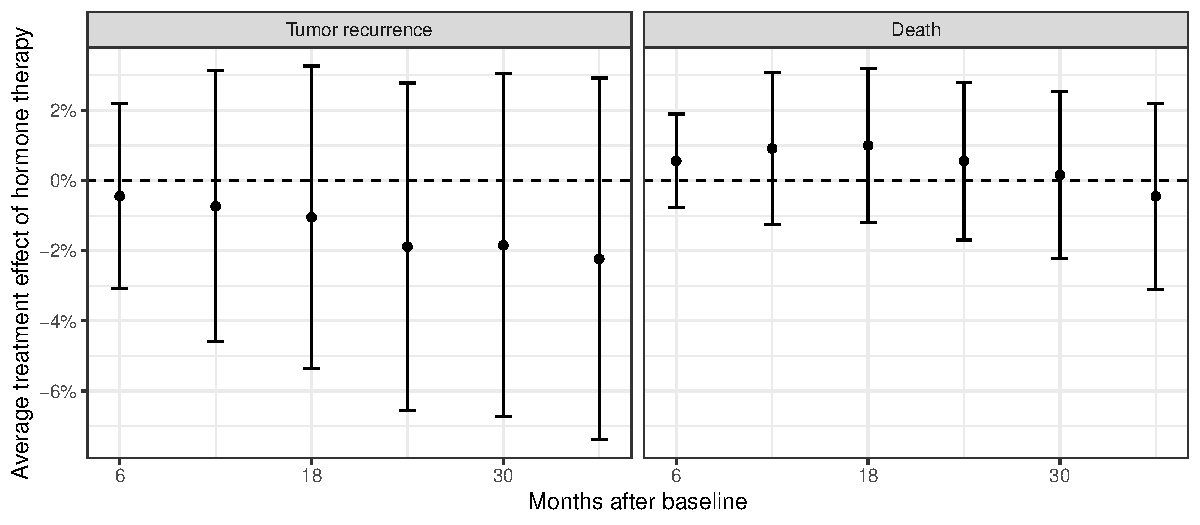
\includegraphics[width=1\linewidth]{real-data-target.pdf}
  \caption[]{Estimates of the average treatment effect of hormone therapy on the
    risk of tumor recurrence and death obtained from the prostate cancer study
    analysed by \cite{kattan2000pretreatment}. The estimates are based on the
    estimator defined in equation~(\ref{eq:one-step-comp-ate}) with pointwise
    95\% confidence intervals calculated as described in
    Section~\ref{sec:targeted-learning}. The estimates of the nuisance
    parameters are provided by the state learner.}
  \label{fig:zelefski-real-target}
\end{figure}


\appendix

\subsection{Transience of the second order remainder structure}
\label{sec:state-learner-with}

Recall that we let $\Lambda_1$ denote the conditional cumulative hazard function
for one of the event times of interest and $\Gamma$ the conditional cumulative
hazard function for censoring, c.f., Section~\ref{sec:framework}.

\begin{proof}[Proof of Proposition~\ref{prop:dr-structure}]
  For notational convenience we suppress \( X \) in the following. The final
  result can be obtained by adding the argument \( X \) to all functions and
  averaging. We use the relations from equation~\eqref{eq:7} to write
  \begingroup %
  \allowdisplaybreaks
    \begin{align*}
      & \int_0^{\tau} w(s) 
        \left\{
        \Gamma(s) - \hat{\Gamma}_n(s)
        \right\}
        [\Lambda_1 - \hat{\Lambda}_{1,n}](\diff s)
      \\
      & =
        \int_0^{\tau} w(s) 
        \left\{
        \int_0^s \frac{F(\diff u, -1)}{F(u-, 0)} -
        \int_0^s \frac{\hat{F}_n(\diff u, -1)}{\hat{F}_n(u-, 0)}  -
        \right\}
        \left[
        \frac{F(\diff s, 1)}{F(s-, 0)}
        - \frac{\hat{F}_n(\diff s, 1)}{\hat{F}_n(s-, 0)}
        \right]
      \\
      & =
        \int_0^{\tau} w(s) 
        \Bigg\{
        \int_0^s 
        \left(
        \frac{1}{F(u-, 0)} -  \frac{1}{\hat{F}_n(u-, 0)}
        \right) F(\diff u, -1)
      \\
      & \qquad\qquad \qquad
        +
        \int_0^s \frac{1}{\hat{F}_n(u-, 0)} 
        \left[
        F(\diff u, -1) - \hat{F}_n(\diff u, -1)
        \right]
        \Bigg\}
      \\
      & \qquad\qquad \times
        \left[
        \left(
        \frac{1}{F(s-, 0)} -
        \frac{1}{\hat{F}_n(s-, 0)}
        \right)F(\diff s, 1)
        + \frac{1}{\hat{F}_n(s-, 0)}
        \left(
        F(\diff s, 1) -
        \hat{F}_n(\diff s, 1)
        \right)
        \right]
      \\
      &
        = \int_0^{\tau} 
        \int_0^s
        w(s) 
        \left(
        \frac{1}{F(u-, 0)} -  \frac{1}{\hat{F}_n(u-, 0)}
        \right) 
        \left(
        \frac{1}{F(s-, 0)} -
        \frac{1}{\hat{F}_n(s-, 0)}
        \right)F(\diff u, -1)F(\diff s, 1)
      \\
      & \quad +
        \int_0^{\tau}
        \int_0^s
        w(s) 
        \left(
        \frac{1}{F(u-, 0)} -  \frac{1}{\hat{F}_n(u-, 0)}
        \right) \frac{F(\diff u, -1) }{\hat{F}_n(u-,0)}
        \left(
        F(\diff s, 1) -
        \hat{F}_n(\diff s, 1)
        \right)
      \\
      & \quad +
        \int_0^{\tau} 
        \int_0^s      
        \frac{w(s) }{\hat{F}_n(u-, 0)} 
        \left[
        F(\diff u, -1) - \hat{F}_n(\diff u, -1)
        \right]
        \left(
        \frac{1}{F(s-, 0)} -
        \frac{1}{\hat{F}_n(s-, 0)}
        \right)F(\diff s, 1)
      \\
      & \quad +
        \int_0^{\tau} 
        \int_0^s      
        \frac{w(s) }{\hat{F}_n(u-, 0)} 
        \left[
        F(\diff u, -1) - \hat{F}_n(\diff u, -1)
        \right]
        \frac{1}{\hat{F}_n(s-, 0)}
        \left(
        F(\diff s, 1) -
        \hat{F}_n(\diff s, 1)
        \right).
    \end{align*}
    \endgroup %
    Consider the first term on the right hand side. By the mean value theorem,
    \begin{equation*}
      \frac{1}{F(t-, 0)}
      - \frac{1}{\hat{F}_n(t-, 0)}
      = \frac{-1}{\tilde{r}_n(t)^2}
      \left[
        F(t-, 0)
        - \hat{F}_n(t-, 0)
      \right],
    \end{equation*}
    where \( \tilde{r}_n(t) \) is some value between \( \hat{F}(t-, 0) \) and
    \( \hat{F}_n(t-, 0) \). Letting \( w_n^*(t) = -\tilde{r}_n(t)^{-2} \), we
    may write
  \begin{align*}
    & \int_0^{\tau} 
      \int_0^s
      w(s) 
      \left(
      \frac{1}{F(u-, 0)} -  \frac{1}{\hat{F}_n(u-, 0)}
      \right)      
      \left(
      \frac{1}{F(s-, 0)} -
      \frac{1}{\hat{F}_n(s-, 0)}
      \right)F(\diff u, -1)F(\diff s, 1)
    \\
    & =
      \int_0^{\tau} 
      \int_0^s
      w(s)
      w_n^*(u) 
      \left(
      F(u-, 0) - \hat{F}_n(u-, 0)
      \right)
    \\
    & \qquad \qquad \quad
      \times
      w_n^*(s) 
      \left(
      F(s-, 0) - \hat{F}_n(s-, 0)
      \right)       
      F(\diff u, -1)F(\diff s, 1)
    \\
    & =
      \int_0^{\tau} 
      \int_0^s
      w_n^a(s,u)
      \left(
      F(u-, 0) - \hat{F}_n(u-, 0)
      \right)
      \left(
      F(s-, 0) - \hat{F}_n(s-, 0)
      \right)       
      F(\diff u, -1)F(\diff s, 1),
  \end{align*}
  where we have defined \( w_n^a(s,u) = w(s)w^*_n(s)w^*_n(u) \). By the
  assumption that \( F(\blank,0) \) and \( F_n(\blank,0) \) are uniformly
  bounded away from zero on \( [0,\tau] \), it follows that \( w_n^* \) is
  uniformly bounded, and hence \( w_n^a(s,u) \) is also uniformly bounded,
  because \( w \) was assumed uniformly bounded. The same approach can be
  applied to the three remaining terms which gives the result.
\end{proof}
